\chapter{General Methodology}\label{ch: general methodology}

This chapter describes the general methods that were applied in the long-read sequencing experiments in \textbf{Chapters 4,6 and 7}. Experimental methods specific to individual results chapters can be found in the Methods section of the relevant chapter. Methods pertaining to the library preparation for PacBio Isoform Sequencing (Iso-Seq) and ONT Nanopore cDNA sequencing can be found in \cref{chap:isoseq_labpipeline} and \cref{chap:ont_labpipeline}. Standard manufacturers protocols used in my thesis can be found in \textbf{Appendix \ref{app_longread_protocol}}. All reagents mentioned in this Chapter were provided with the respective kits unless otherwise stated.

\section{Mouse tissue samples and isolation of nucleic acids}

\subsection{Mouse model of AD tauopathy: rTg4510} 
rTg4510 mice recapitulate AD tauopathy through the overexpression of the human tau transgene, MAPT\textsuperscript{P301L}, which harbours the FTD-associated P301L mutation. It contains four microtubule-binding domains while lacking the N-terminal segment (4R0N), and exons 2-3 of the mouse prion protein gene \textit{Prnp}. The transgene expression is controlled under the calcium calmodulin kinase II promoter (CaMK2a) and is largely restricted to the forebrain, with age-dependent spread of neuropathology starting from as early as 2 months in the neocortex and progressing rapidly to the hippocampus by 5 months. Neuronal and synaptic loss is also observed by 9 months, with these mice exhibiting cognitive and behavioural impairments. Sex differences in pathology have been reported with female mice exhibiting earlier and more severe cognitive and behavioural impairments than transgenic male mice\cite{M2011}. The rTg4510 mouse model is particularly informative as tau expression is induced through the tetracycline operon-responsive element and suppressed after doxycycline treatment\cite{Ramsden2005}. However, a study in 2019 reported disruption of several endogenous mouse genes in this model due to the random integration of MAPT\textsuperscript{P301L}, which has additional off-target effects that potentially contribute to the neurodegenerative phenotype associated with rTg4510\cite{Gamache2019}. 
 

\subsection{Animal breeding \& Sample Preparation}
\label{sec: animalbreeding_sample preparation}
All animal procedures were carried out at Eli Lilly and Company, in accordance with the UK Animals (Scientific Procedures) Act 1986 and with approval of the local Animal Welfare and Ethical Review Board. All mice were bred and delivered to Eli Lilly and Company (Windlesham, UK) by Envigo (Loughborough, UK), where animals were housed under standard conditions (constant temperature and humidity with a 12h light/dark cycle in individually ventilated cages) before terminal anaesthesia with pentobarbital and transcardial perfusion with phosphate-buffered saline (PBS)\cite{Castanho2020}

The entorhinal cortex was dissected from the left-brain hemisphere of female transgenic mice (TG\nomenclature{TG}{Transgenic mice}) and wild-type controls (WT\nomenclature{WT}{Wild-type mice}), aged 2, 4, 6 and 8 months (n = 9-10 mice per group). Total RNA was then extracted\cite{Castanho2020} using the AllPrep DNA/RNA Mini Kit (Qiagen) according to the manufacturer's protocol, and converted to complementary DNA (cDNA) for library preparation (described later in \cref{section:ch2_cDNA_synthesis_explanation}). Of note, >80\% of total RNA is comprised of ribosomal RNA, 15\% of tRNA, with only 1-5\% of representing mRNA. 

\subsection{Assessment of nucleic acid quality and quantity}
Acquiring high-quality RNA, successful cDNA synthesis and multi-step library preparation are all crucial for optimal sequencing experiments, particularly for long-read sequencing. The assessment of the purity and integrity of extracted RNA, followed by cDNA quality and quantity, was therefore required throughout the library preparation and quality control (QC) stages of my sequencing experiments. This was undertaken using the RNA/DNA ScreenTape and Bioanalyzer assays for qualitative assessment, and the Qubit for DNA quantification. 


\subsection{ScreenTape \& Bioanalyzer}
\label{section:ch2_bioanalyzer} 
ScreenTape and Bioanalyzer assays are commonly used to provide an accurate, automated assessment of nucleic acid quality and size by electrophoresis. It works on the principle that upon applying an electric field, negatively-charged DNA migrates through a gel matrix towards the positive anode at a rate that is dependent on DNA size; smaller DNA fragments migrate faster, and thus move further through the gel within a specific time frame. The separated DNA can be then visualised using a fluorescent dye that intercalates into the double-stranded DNA (dsDNA\nomenclature{dsDNA}{double-stranded DNA}) structure and fluoresces under ultraviolet light. 

Both RNA ScreenTape and Bioanalyzer assays further provide a numeric evaluation of the quality of an RNA sample using a score between 1 and 10 - this is known as a RNA Integrity Number (RIN\nomenclature{RIN}{RNA Integrity Number} - with 1 indicative of high degradation and poor quality RNA, and 10 indicative of minimal degradation (Figure \ref{fig:bionalayzer_pics}). The purity and quantity of extracted RNA was assessed using the RNA Bioanalyzer assay with Agilent RNA 6000 Nano Kit (Agilent Technologies) and Agilent 2100 Bioanalyzer instrument (Agilent Technologies). 

Given that the Bioanalyzer assay is more sensitive than the ScreenTape assay, assessment of cDNA quality during various QC stages of long-read library preparation was mostly performed using the DNA Bioanalyzer assay with Agilent D1200 Kit (Agilent Technologies), particularly where accurate determination of library molarity was critical. However in QC stages where assessment is optional, the D5000 ScreenTape (Agilent Technology) and 4200 TapeStation (Agilent Technology) was used instead as it is cheaper and quicker to run than the Bioanalyzer. Both assays were performed following the standard manufacturer's protocol. Briefly, this involved mixing the sample with the ladder and buffer if using the ScreenTape, or with the marker and gel-dye mix if using the Bioanalyzer assay, before loading the sample into the machine to be assayed. Detailed lab instructions for Bioanalyzer and ScreenTape assays are detailed in \textbf{Appendix \ref{Isoseq_Protocol_tapestation_bioanalyzer}}.  

\begin{figure}[htp]
	\centering
	\vspace{20pt}
	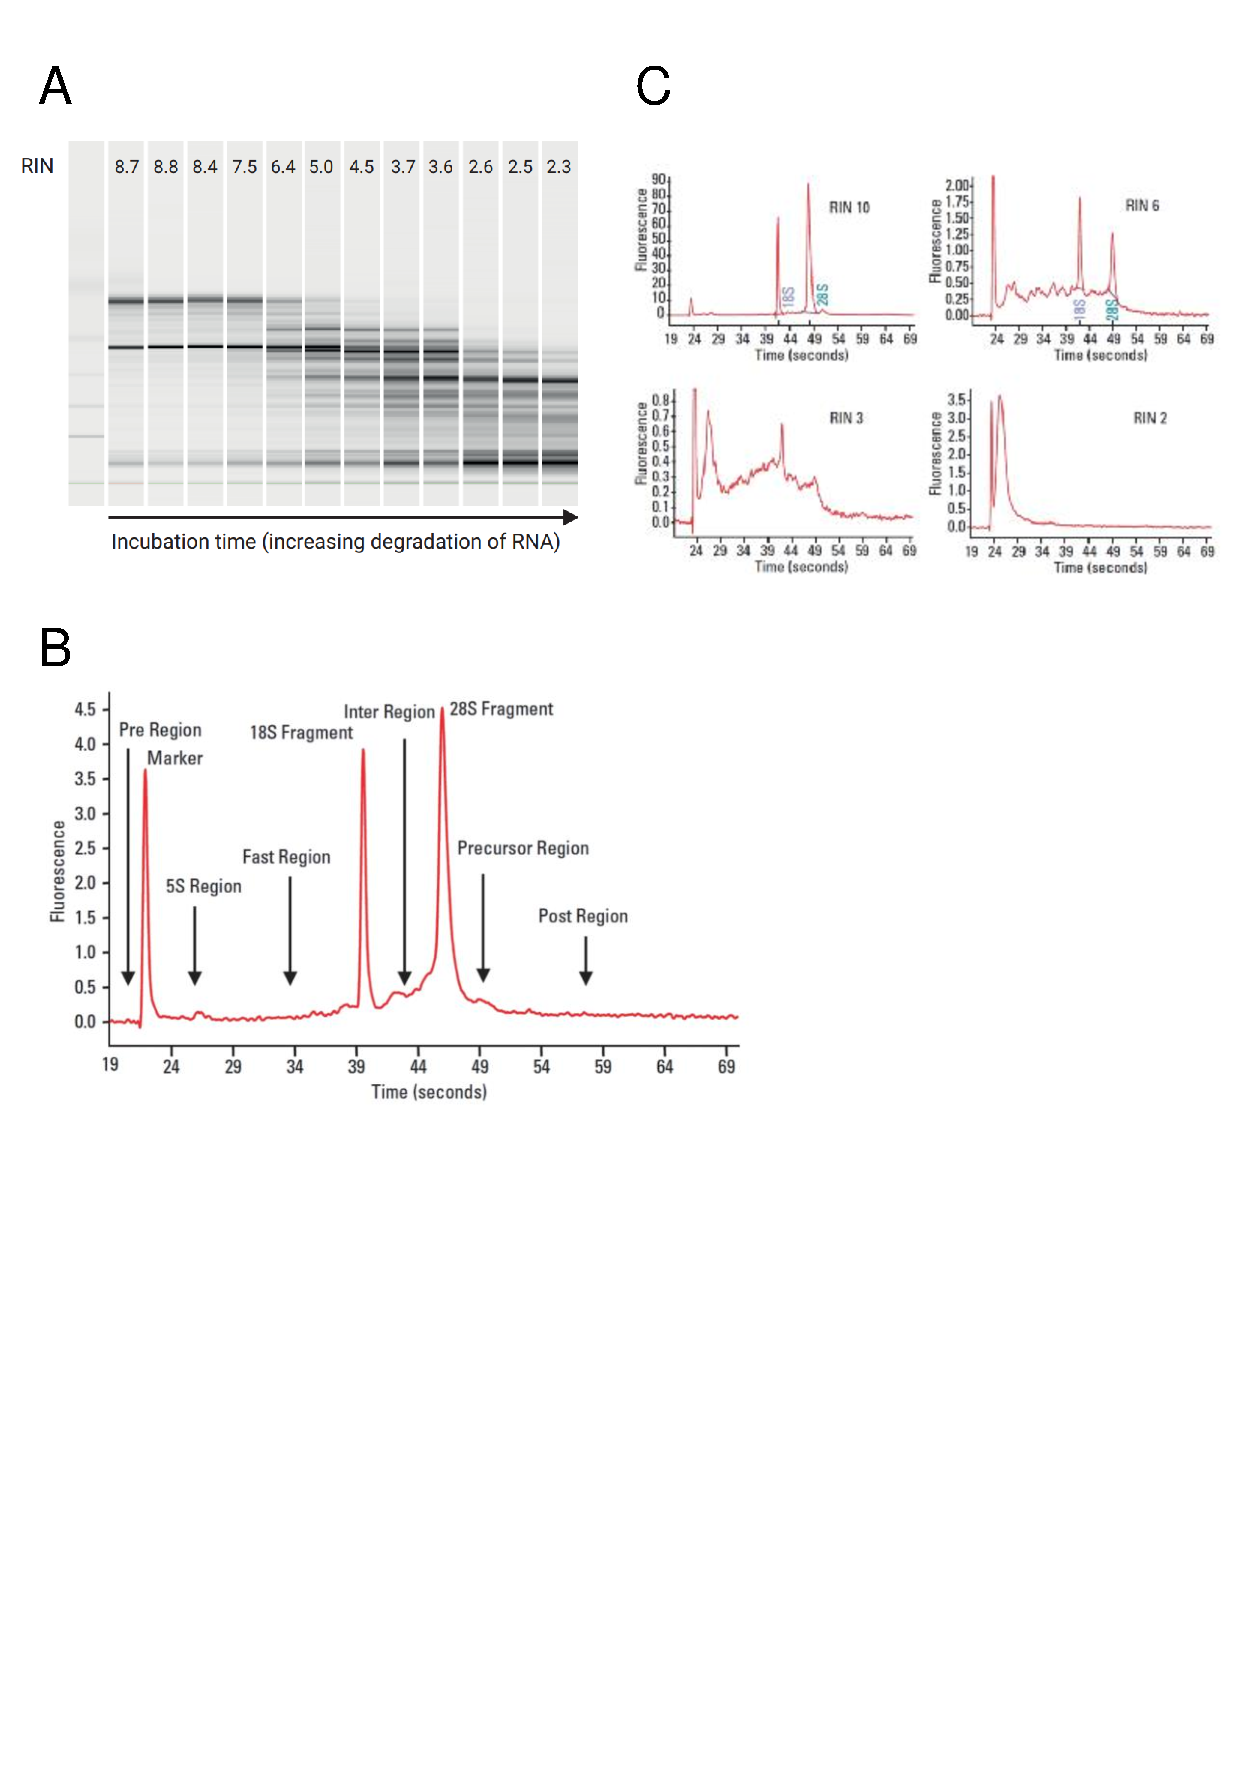
\includegraphics[page=1,trim={0 10cm 0 0 },clip, scale = 0.7]{Figures/General_Methodology_Figures.pdf}
	\captionsetup{width=0.95\textwidth}
	\caption[Evaluation of RNA integrity with Bioanalyzer and TapeStation]%
	{\textbf{Evaluation of RNA integrity with Bioanalyzer and TapeStation}: \textbf{a)} A Bioanalyzer electropherogram showing progressive total RNA degradation over prolonged incubation time with a general shift towards more bands representing shorter fragments. \textbf{b)} The degree of degradation is represented by a RNA integrity number (RIN), ranging from intact (RIN = 10) to degraded (RIN = 2) RNA, and is calculated by the relative ratio of the fast region and 18S, 28S fragment (Figure c). Figures and legends are adapted from Mueller et al. 2016.}
	\label{fig:bionalayzer_pics}
\end{figure}

\subsection{Qubit}
\label{section:ch2_qubit}   
Qubit assays (Invitrogen) allow accurate nucleic acid quantification by the selective binding of fluorescent Qubit dyes to dsDNA or RNA, making it more sensitive and specific than the UV absorbance used in NanoDrop 8000 spectrophotometer (Thermo Fisher Scientific). Following RNA isolation, the RNA concentration was determined using Qubit assays to ensure that the same amount of total RNA for each sample was used for library preparation. Many of the QC steps post DNA purification (later discussed in \cref{section:ch2_AMPure_explanation}) throughout library preparation also required Qubit assays to determine the cDNA concentration prior to proceeding with downstream experiments. This involved first preparing two 'standard samples' with Qubit reagent in 10:200 ratio, and 'test samples' with the same reagent in a 1:200 ratio, before placing and running the samples on the Qubit 3.0 Fluorometer (Thermo Fisher Scientific) using the standard manufacturer's protocol as detailed in \textbf{Appendix  \ref{Isoseq_Protocol_qubit}}.       

\section{cDNA synthesis, amplification \& purification}
After RNA isolation, integrity assessment and quantification, total RNA was converted to cDNA. Given that mRNA only typically accounts for <5\% of total RNA and the low sensitivity of current sequencing platforms, cDNA was subsequently amplified using Polymerase Chain Reaction (PCR\nomenclature{PCR}{Polymerase Chain Reaction}) and assessed using agarose gel electrophoresis. 


\subsection{Complementary DNA synthesis}
\label{section:ch2_cDNA_synthesis_explanation} 
As recommended as part of the Iso-Seq protocol, the SMARTer PCR cDNA Synthesis Kit (Clontech) was used to convert 200ng total RNA to cDNA (outlined in \cref{fig:cDNAsynthesis_workflow}). In brief, the polyA tails of mRNA transcripts were first primed by a modified oligo (dT) primer to allow first-strand cDNA synthesis by SMARTScribe Reverse Transcriptase to generate a first single-stranded DNA, which was then diluted and subsequently amplified \cite{Ramskold2012}. Detailed instructions of the lab workflow can be found in \textbf{Appendix \ref{Isoseq_protocol_cDNAsynthesis}}. 

In order to sequence samples simultaneously (i.e. in “multiplex”), as used for my targeted sequencing experiments, unique barcoded oligo (dT) primer was used in place of the standard oligo (dT) primer (\cref{tab:barcode_primers}). PacBio recommends multiplexing 6 - 8 samples per run.

While this kit is advantageous in preferentially enriching for full-length cDNA sequences, it cannot differentiate between intact and truncated RNA. As truncated RNA is present in poor-quality samples it will be amplified as a potential source of contamination in the final cDNA library. One alternative is to exploit the 5’-cap that is present only in intact RNA and not truncated RNA (5-cap refers to the addition of 7-methylguanosine to the 5’ end of mRNA during transcription, to protect nascent mRNA from degradation and assist in protein translation). The use of alternative reverse transcriptases have been explored that only converts 5’capped mRNAs to cDNA, however, these have been found to negatively influence read length on the ONT platform\cite{Cartolano2016}. An alternative method, Full-Length cDNA Amplification (Teloprime)\cite{Cartolano2016}, relies on a double-stranded adapter that recognises and ligates to the 5’cap at the end of first strand synthesis (\textbf{Appendix \ref{ch:alt_cDNA}}).

\begin{figure}[htp]
	\centering
	\vspace{20pt}
	\includegraphics[page=2,trim={0 12cm 0 0 },clip, scale = 0.7]{Figures/General_Methodology_Figures.pdf}
	\captionsetup{width=0.95\textwidth,singlelinecheck=off}
	\caption[Flowchart of SMARTer cDNA synthesis]%
	{\textbf{Flowchart of SMARTer cDNA synthesis}: SMARTer cDNA synthesis ensures the generation of full-length cDNA by the usage of the enzyme terminal transferase activity, whereby premature termination of RT results in less efficient transferase activity, and subsequent absence of overhang for downstream amplification. 
	cDNA synthesis is achieved in the following manner: 
	\begin{enumerate}
		\item Oligo(dT) primer (3’ SMART CDS Primer II A) primes the first-strand synthesis reaction by binding to polyA tail and transcribes the RNA into single-stranded DNA
		\item As RT reaches the 5’ end of the mRNA, the enzyme’s terminal transferase activity adds a few additional nucleotides to the 3’ end of the cDNA
		\item With a 3’end that is complementary to the added nucleotides, the SMARTer Oligonucleotide, or the template switching oligo, base-pairs with it and creates an extended template.
		\item RT then switches templates and continues transcribing to the end of the SMARTer oligonucleotide 
		\item The resulting full-length, single-stranded (ss) cDNA contains the complete 5’ end of the mRNA, as well as a 3’ end that is complementary to the SMARTer Oligonucleotide. 
		\item The SMARTer Oligonucleotide and the poly A sequence then serves as universal priming sites for end-to-end cDNA amplification.
		\\
		
	\end{enumerate}
	Of note, the SMARTer II A Oligonucleotide, 3’ SMART CDS Primer II A, and 5’ PCR Primer II A all contain a stretch of identical sequence.  

	Figure is taken from the SMARTer PCR cDNA Synthesis Kit User Manual. RT - Reverse Transcriptase.
	}
	\label{fig:cDNAsynthesis_workflow}
\end{figure}


\begin{landscape}
	The general structure of the barcoded oligo-dT primer is as follows:
	\\
	\\
	\hangindent=5cm \textcolor{RedOrange}{Primer Sequence} \hspace{2cm}   \textcolor{ForestGreen}{16-bp barcode}   \hspace{4cm} \textcolor{RoyalBlue}{oligo-dT}
	\begin{center}
		5'\textcolor{RedOrange}{AAGCAGTGGTATCAACGCAGAGTAC}\textcolor{ForestGreen}{tcagacgatgcgtcat}\textcolor{RoyalBlue}{TTTTTTTTTTTTTTTTTTTTTTTTTTTTTTVN3’}
	\end{center}
	\vspace{1cm}

	\begin{table}[ht]
		\captionsetup{justification=raggedright,width=1.45\textwidth}
		\caption[Barcoded Oligo-dT Primers for targeted transcriptome sequencing]%
		{\textbf{Barcoded oligo-dT primers were used for multiplexing samples in targeted transcriptome sequencing}. Each of the barcoded primers contain the same 5' primer sequence and oligo-dT for reverse transcription of first strand cDNA synthesis using Clontech kit SMARTer PCR cDNA Synthesis Kit. The different internal 16bp sequence allows tagging and differentiation of samples in the same sequencing run. The barcodes are recommended from official PacBio's multiplex protocol.}
		\label{tab:barcode_primers}
		\begin{tabularx}{1.45\textwidth}{ll}
			\toprule
			Barcode Name & Sequence                                                                  \\ \midrule
			Barcode 1    & AAGCAGTGGTATCAACGCAGAGTACCACATATCAGAGTGCGTTTTTTTTTTTTTTTTTTTTTTTTTTTTTTVN \\
			Barcode 2    & AAGCAGTGGTATCAACGCAGAGTACACACACAGACTGTGAGTTTTTTTTTTTTTTTTTTTTTTTTTTTTTTVN \\
			Barcode 3    & AAGCAGTGGTATCAACGCAGAGTACACACATCTCGTGAGAGTTTTTTTTTTTTTTTTTTTTTTTTTTTTTTVN \\
			Barcode 4    & AAGCAGTGGTATCAACGCAGAGTACCACGCACACACGCGCGTTTTTTTTTTTTTTTTTTTTTTTTTTTTTTVN \\
			Barcode 5    & AAGCAGTGGTATCAACGCAGAGTACCACTCGACTCTCGCGTTTTTTTTTTTTTTTTTTTTTTTTTTTTTTTVN \\
			Barcode 6    & AAGCAGTGGTATCAACGCAGAGTACCATATATATCAGCTGTTTTTTTTTTTTTTTTTTTTTTTTTTTTTTTVN \\
			Barcode 7    & AAGCAGTGGTATCAACGCAGAGTACTCTGTATCTCTATGTGTTTTTTTTTTTTTTTTTTTTTTTTTTTTTTVN \\
			Barcode 8    & AAGCAGTGGTATCAACGCAGAGTACACAGTCGAGCGCTGCGTTTTTTTTTTTTTTTTTTTTTTTTTTTTTTVN \\
			Barcode 9    & AAGCAGTGGTATCAACGCAGAGTACACACACGCGAGACAGATTTTTTTTTTTTTTTTTTTTTTTTTTTTTTVN \\
			Barcode 10 & AAGCAGTGGTATCAACGCAGAGTACACGCGCTATCTCAGAGTTTTTTTTTTTTTTTTTTTTTTTTTTTTTTVN \\ \bottomrule
		\end{tabularx}
	\end{table}
\end{landscape}


\subsection{Polymerase Chain Reaction (PCR)}
\label{section:ch2_PCR_explanation} 
PCR is a well-established method for generating multiple copies of the same DNA sequence. Mimicking natural DNA replication, this relies on a thermostable DNA polymerase, a set of primers specific to the region of interest, and a cocktail of various reagents required for polymerisation (such as deoxynucleotides\nomenclature{dNTPs}{Deoxynucleotides}, buffers). This reaction is subjected to a series of heating and cooling steps: 
\begin{enumerate}
	\item Denaturation at 96$^{\circ}$C, to separate any dsDNA 
	\item Annealing, typically between 55$^{\circ}$C  and 65$^{\circ}$C, for the binding of primers to the complementary sequences on the ssDNA; the specific annealing temperature is dependent on the primer sequence. 
	\item Extension at 72$^{\circ}$C to allow the polymerase to extend the primers, consequently synthesising a new cDNA strand using dNTPs
\end{enumerate} 
These three steps are then repeated multiple times, or "cycles", resulting in an exponential generation of the DNA template of interest.

\subsection{Agarose Gel Electrophoresis}
\label{section:ch2_agarose_explanation}  
Agarose gel electrophoresis allows the separation of dsDNA molecules based on length, and works on the same principle as the Bioanalyzer and ScreenTape assays described above. It is most commonly used to determine DNA quality and quantity, and assess the efficiency of molecular biology techniques such as PCR amplification in determining the number of optimum cycles. It is well known that increased number of PCR cycles an generate artefacts (strand invasion) and preferential amplification of shorter transcripts\cite{Acinas2005,Bayega2018}. Instructions to set up and run an agarose gel electrophoresis are detailed in \textbf{Appendix \ref{Isoseq_Protocol_running_agarose_gel}}.


\subsection{AMPure Bead Purification} 
\label{section:ch2_AMPure_explanation} 
At various stages of long-read library preparation, cDNA was purified using AMPure beads (\cref{fig:ampure_bead_workflow}\textbf{a}). These are paramagnetic beads that reversibly bind to DNA in the presence of polyethylene glycol (PEG) and salt. The concentration of PEG, and consequent ratio of beads to DNA, determines the size of fragments that are bound and subsequently eluted (\cref{fig:ampure_bead_workflow}\textbf{b}); the lower the concentration of beads to DNA, the greater the proportion of longer DNA fragments bound. This is because beads will preferentially bind to larger molecular weight DNA with a higher negative charge, resulting in attachment of longer fragments and displacement of shorter fragments; a 0.4X AMPure bead concentration would therefore retain only the larger DNA fragments whereas a 1X AMPure bead concentration would retain both long and short DNA fragments (\cref{fig:ampure_bead_workflow}\textbf{b}). Briefly, AMPure Bead purification was performed by thoroughly mixing and vortexing each sample with a pre-specified ratio of AMPure Bead, placing the sample on a magnet for clearer separation of DNA-bound beads and solution, followed by two washes of 70\% ethanol and DNA elution. Detailed instructions can be found in \cref{general_ampure_bead_purification}.

\begin{figure}[!h]
	\centering
	\vspace{20pt}
	\includegraphics[page=3,trim={0 8cm 0 0 },clip, scale = 0.7]{Figures/General_Methodology_Figures.pdf}
	\captionsetup{width=0.95\textwidth}
	\caption[Overview lab workflow of DNA purification with AMPure Beads]%
	{\textbf{Overview lab workflow of DNA purification with AMPure Beads}: A schematic figure depicting \textbf{a)} steps of purifying DNA with AMPure Beads, with initial binding of magnetic beads to negatively-charged DNA enabling separation of DNA fragments, followed by ethanol wash and elution. \textbf{b)}) An agarose gel image of DNA purified using a range of bead to DNA ratio. As shown, size selection is achieved with different ratios, with a lower ratio retaining only longer fragments. Figures are taken from Beckman Website. Detailed instructions of the workflow can be found in \textbf{Appendix \ref{general_ampure_bead_purification}}}
	\label{fig:ampure_bead_workflow}
\end{figure}

\clearpage
\section{ERCC-RNA Spike-In Controls}
\label{section:ch2_ERCC_explanation} 
To evaluate the performance of library preparation and the sequencing experiments, and to validate the Iso-Seq pipeline to accurately characterise the transcriptome using long reads, a set of external RNA Spike-In controls, generated by the External RNA Controls Consortium (ERCC\nomenclature{ERCC}{External RNA Controls Consortium}), was used. ERCC consists of 92 polyadenylated synthetic transcripts (250 to 2000 nucleotides) of known sequences from the ERCC plasmid library, which are added in pre-determined amounts to the sample prior to first-strand cDNA synthesis. The addition of ERCC allowed me to assess the quantitative power of long-read sequencing in addition to providing absolute quantification of mRNA isoforms with the sample by generating a standard curve. It can further validate that the bioinformatics pipeline only identifies 1 isoform per ERCC gene. 

The amount of spike-in control was calculated using the below equation \cite{WTAC}:
\begin{myequation}[!h]
	\begin{equation}
		\label{eqn:ercc_calcaluations}
		mass_{RNA spike} = fraction_{spiked reads}\; * fraction_{target RNA}\; *mass_{RNA input}
	\end{equation}
	\begin{equation}
		concentration_{RNA spike} = mass_{RNA spike}\; * volume_{RNA spike}
	\end{equation}
	where:
	\begin{conditions*}
		mass_{RNA spike} & mass of RNA spike-in to be added to sample \\
		concentration_{RNA spike} & final diluted concentration (ngs/ul) of the RNA spike-in \\
		fraction_{spiked reads}  &   desired proportion of sequenced spike-in RNA reads relative to total amount of sequenced reads \textit{(3\%)} \\
		fraction_{target RNA}    &  expected proportion of target RNA, in this case mRNA relative to total RNA \textit{(3\%)} \\   
		mass_{RNA input} &  input of total RNA \textit{(200ng)} \\
		volume_{RNA spike} & volume of RNA spike-in \textit{(0.1uL)}				
	\end{conditions*}
	\captionsetup{width=0.95\textwidth}
	\caption[Determining amount of ERCC-RNA Spike-In Control]%
	{\textbf{Determining amount of ERCC-RNA Spike-In Control}. In determining the mass and final concentration of RNA-spike-in mix based on the above conditions, the stock ERCC RNA spike-in was diluted from the original concentration of 30ng/$\mu$L to 1.8ng/$\mu$L with a dilution factor of 1:16.8. The italicised parameters were taken from the RNA Transcriptomics 2018 Course\cite{WTAC} with the exception of total RNA input}
\end{myequation}

A separate pilot experiment (Appendix \ref{ch:alt_cDNA}) showed successful addition of ERCC with two main bands at \textasciitilde600bp and \textasciitilde1000bp (Figure \ref{fig:ercc_lab_gel}a), reflecting significant enrichment of ERCC transcripts at these two respective lengths as is expected (Figure \ref{fig:ercc_lab_gel}b). The stark contrast of these two bands, however, to the smear of cDNA, suggests that the ERCC transcripts are predominant - this could be due to an overestimation of assumed proportion of mRNA to total RNA, which is likely in reality to be lower than 3\%. To reduce unnecessary sequencing and coverage of ERCC transcripts, a lower ERCC RNA-spike in concentration was used (final concentration of 0.6ng/$\mu$L and a dilution factor of 1:50.5, Figure \ref{fig:ercc_lab_gel}c). 

\begin{figure}[!htp]
	\begin{center}
		\includegraphics[page=4,trim={0 8cm 0 2cm},clip,scale = 0.65]{Figures/General_Methodology_Figures.pdf}
	\end{center}
	\captionsetup{width=0.95\textwidth}
	\caption[ERCC usage to benchmark library preparation and sequencing performance runs]%
	{\textbf{Successful addition of ERCC to first-strand cDNA synthesis a)}. Agarose gel image taken from PCR amplification of cDNA and ERCC (1.8ng/$\mu$L determined from equation \ref{eqn:ercc_calcaluations}), and ERCC alone as a positive control. 5$\mu$L of PCR aliquots were taken every cycle (13 - 18) and then run on gel electrophoresis. The two bands at 600bp and 1000bp refer to the enrichment of ERCC transcripts at these two lengths as would be expected. \textbf{b)} Distribution of known ERCC length, with a significant proportion of transcripts sized at 500-600bp and 1000-1200bp. \textbf{c)} Agarose gel image after a repeat of PCR amplification of cDNA and ERCC at a lower concentration (0.6ng/$\mu$L), ERCC as positive and water as negative control respectively. The numbers above the lane refer to the number of cycles, L denotes to 100bp Ladder.}
	\label{fig:ercc_lab_gel}
\end{figure}
 
